% Derived from week_1 tabular-classification-report/assets/report_template.tex:
% ACM sigconf double columns, booktabs, graphicx, xeCJK, Windows CJK fonts,
% and introduction/data/method/results/discussion/conclusion structure.
% Self-contained source: title, abstract, and content are included below.
% XeLaTeX: compile until cross-references stabilize (normally three passes).
\documentclass[sigconf]{acmart}
\usepackage{booktabs}
\usepackage{graphicx}
\usepackage{float}
\usepackage{xeCJK}
\setCJKmainfont{SimSun}[BoldFont=SimHei,ItalicFont=KaiTi,AutoFakeBold=2]
\setCJKsansfont{SimHei}[BoldFont=SimHei,AutoFakeBold=2]
\setCJKmonofont{SimSun}
\AtBeginDocument{\setlength{\parindent}{2em}}
\setcopyright{none}
\settopmatter{printacmref=false}
\renewcommand\footnotetextcopyrightpermission[1]{}
\fancypagestyle{plain}{\fancyhf{}\fancyfoot[C]{\thepage}\renewcommand{\headrulewidth}{0pt}}
\begin{document}
\title{多用户电力负荷预测实验}
\author{实验项目技术报告}
\begin{abstract}
本报告比较四种编码器在共同日周期残差框架下的电力负荷预测。使用 370 用户的 2014 年数据，以过去 96 个 15 分钟点预测未来 96 点，在 61 个测试起点评测。CNN 的 1 小时和 24 小时 MAE 分别为 47.174 和 44.064 kW；Transformer 的 6 小时 MAE 为 38.727 kW。结果仅适用于本次单种子设置。
\end{abstract}
\maketitle
\pagestyle{plain}
\suppressfloats[t]




\section{引言}
本实验使用相同数据和预测头比较 CNN、GRU、Transformer 与纯 PyTorch Mamba 编码器，并报告复制前一天负荷的未训练基线。实际运行入口为 \path{src/run.py}，配置为 \path{configs/config.json}，结果和图表位于 \path{results/}。
\section{数据集}
数据为 UCI ElectricityLoadDiagrams20112014，实验取 2014 年全部 370 个用户，每 15 分钟记录功率（kW）。每个样本以过去 96 点预测未来 96 点，输入和输出均为 $96\times370$。按目标时间先后划分，训练、验证、测试分别有 965、61、61 个窗口；训练起点每 6 小时，验证与测试每 24 小时。目标区间不重叠，验证和测试输入可使用起点之前的历史。窗口索引见 \path{results/*_windows.csv}，数据审计见 \path{results/raw_audit.json}。
\section{方法与实验设置}
仅用训练期计算各用户标准化参数，标准差下限为 1 kW。四种编码器共同采用 370 至 32 维输入投影、预测头及前一天负荷残差，种子 42，AdamW 学习率 0.001、批量 32、20 轮、CPU 线程 4；按验证集反标准化 MAE 选择权重。CNN 使用两层时间卷积，GRU 使用单层递归网络，Transformer 使用单层四头注意力，Mamba 使用项目内的纯 PyTorch 实现。具体参数及时间边界见 \path{configs/config.json} 和 \path{results/protocol.json}。
\section{实测结果}
表~\ref{tab:mae} 来自 \path{results/metrics.csv}，四舍五入到三位小数。1、6、24 小时分别为第 4、24、96 个预测点，对 61 个起点及 370 个用户的绝对误差等权平均；全天指标还对全部 96 点平均。指标均为反标准化后的 kW。
\begin{table}[H]
\caption{测试集 MAE（kW，越低越好）。}\label{tab:mae}
\centering\small
\begin{tabular}{lrrrr}\toprule
模型 & 1h & 6h & 24h & 全天 \\
\midrule
前一天复制 & 48.788 & 39.141 & 46.258 & 59.349 \\
CNN & 47.174 & 38.964 & 44.064 & 56.705 \\
GRU & 47.940 & 39.214 & 44.600 & 57.510 \\
Transformer & 47.960 & 38.727 & 44.495 & 56.859 \\
Mamba & 47.819 & 39.590 & 45.475 & 57.763 \\
\bottomrule\end{tabular}
\end{table}
图~\ref{fig:horizon} 展示全部 96 个预测步的误差，图~\ref{fig:forecast} 展示按训练数据选定的 MT\_271 用户首个测试日曲线。图源位于 \path{results/figures/}，文件名分别为 \path{mae_horizon.png} 和 \path{forecast_day.png}；完整预测见各模型 \path{predictions.npz}。




\begin{figure}[htbp]
\centering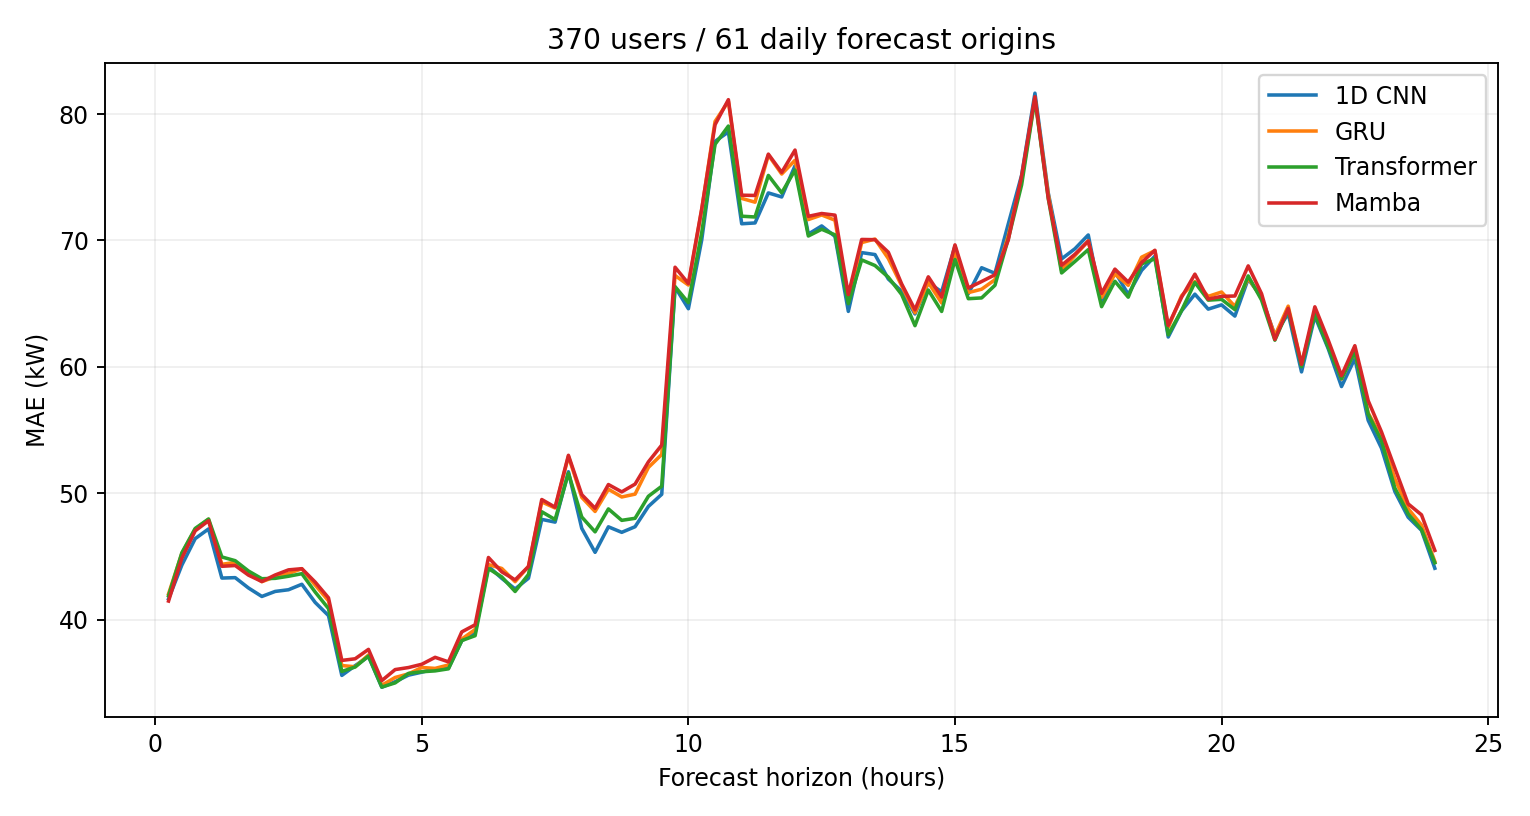
\includegraphics[width=\linewidth]{figures/mae_horizon.png}
\caption{各模型在全部 96 个预测步上的测试 MAE。}\label{fig:horizon}
\end{figure}
\begin{figure}[htbp]
\centering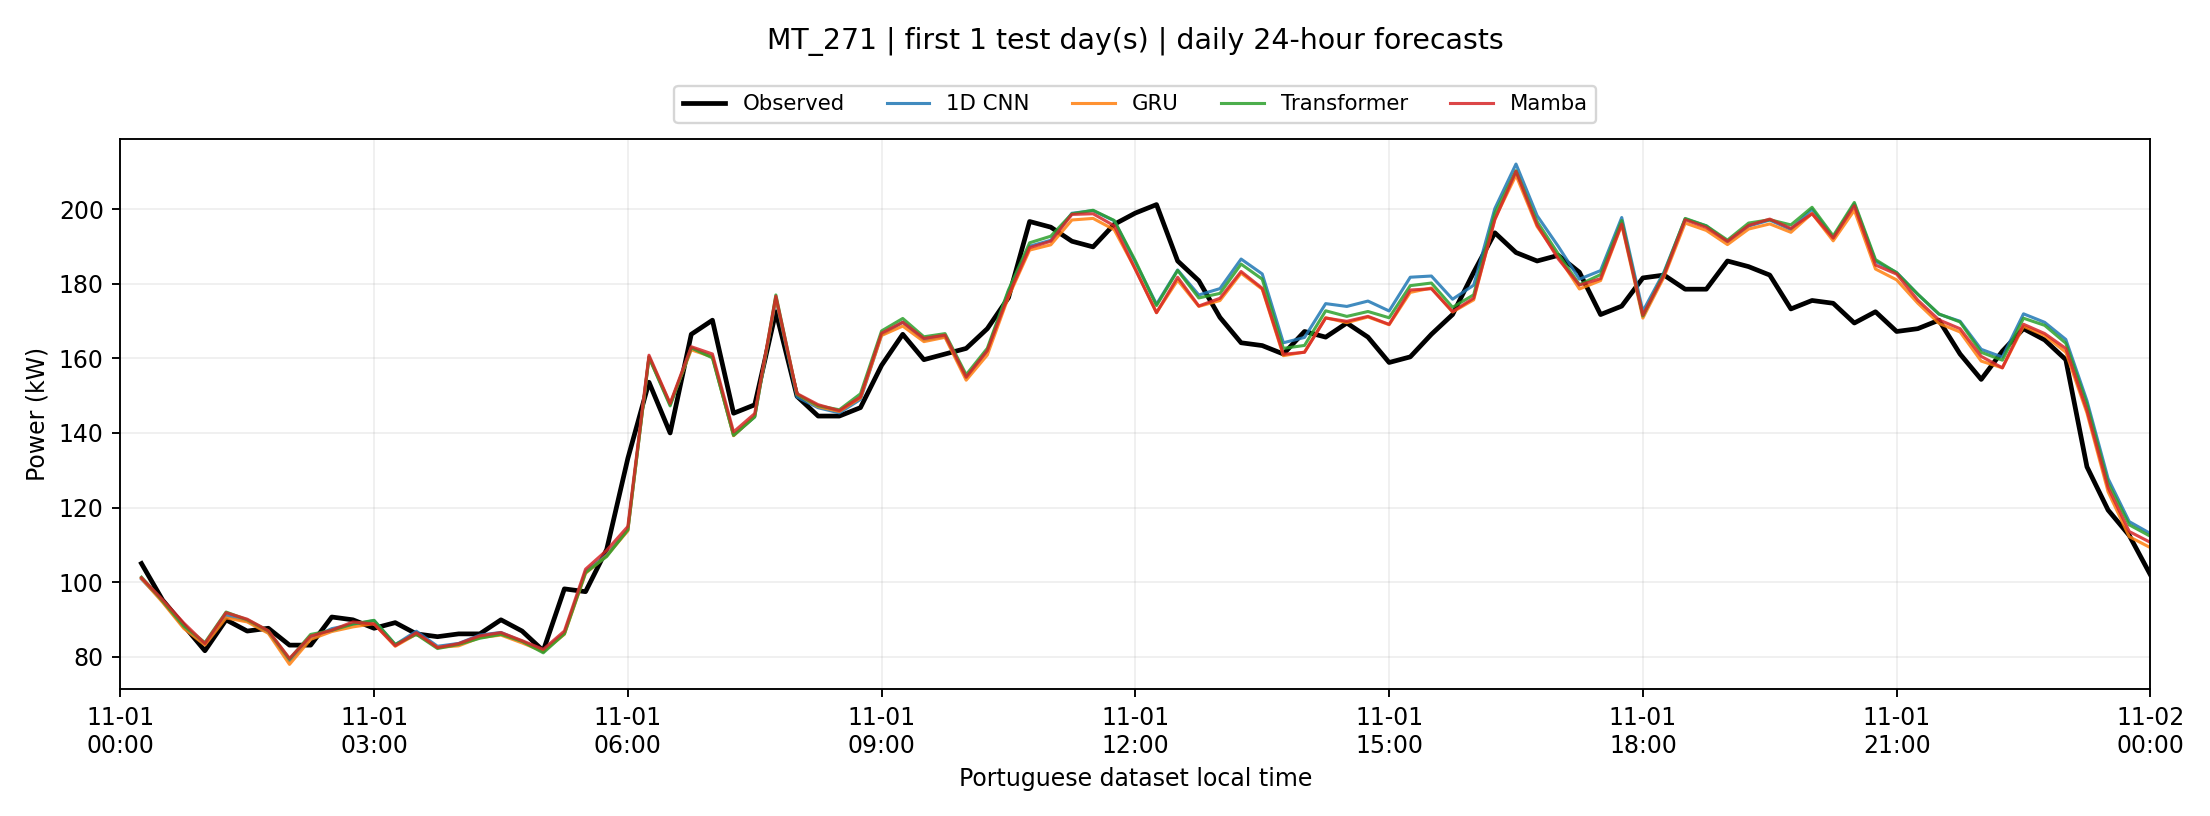
\includegraphics[width=\linewidth]{figures/forecast_day.png}
\caption{MT\_271 首个测试日的实际与预测负荷。}\label{fig:forecast}
\end{figure}
\section{讨论}
CNN 在四个神经模型中取得最低 1 小时、24 小时和全天误差，Transformer 的 6 小时误差最低。测试起点均为午夜，预测距离同时对应不同日内时刻，误差差异不能仅解释为时距影响。图~\ref{fig:forecast} 仅展示一个用户的一天，不能代表全部用户；四模型均共享前一天残差基底。

本次仅使用 2014 年、单随机种子、小模型和一天历史；训练标准化损失与最终 kW 指标的权重不同。未对夏令时与零值做领域修复，CPU Mamba 耗时也不能代表 GPU 融合实现。更广泛结论需要额外实验。
\section{结论}
在本次设定下，CNN 的全天 MAE 为 56.705 kW，低于前一天复制基线的 59.349 kW；这不意味着该模型家族在其他划分或设置中必然领先。
\end{document}
